\subsection{part c}
Now we design feedforward controller to make staedy state error zero.
$$
\lim_{s\to0} \dfrac{s+1}{s^2-2s+4} = 4 \to F(s) = 4
$$
With this controller staedy state is zero and with lead controller (that we have digened in part d) we achive requirements.
\newpage
\begin{itemize}
	\item all figures from siso toolbox
	\begin{figure}[H]
		\caption{All figures from siso toolbox}
		\centering
		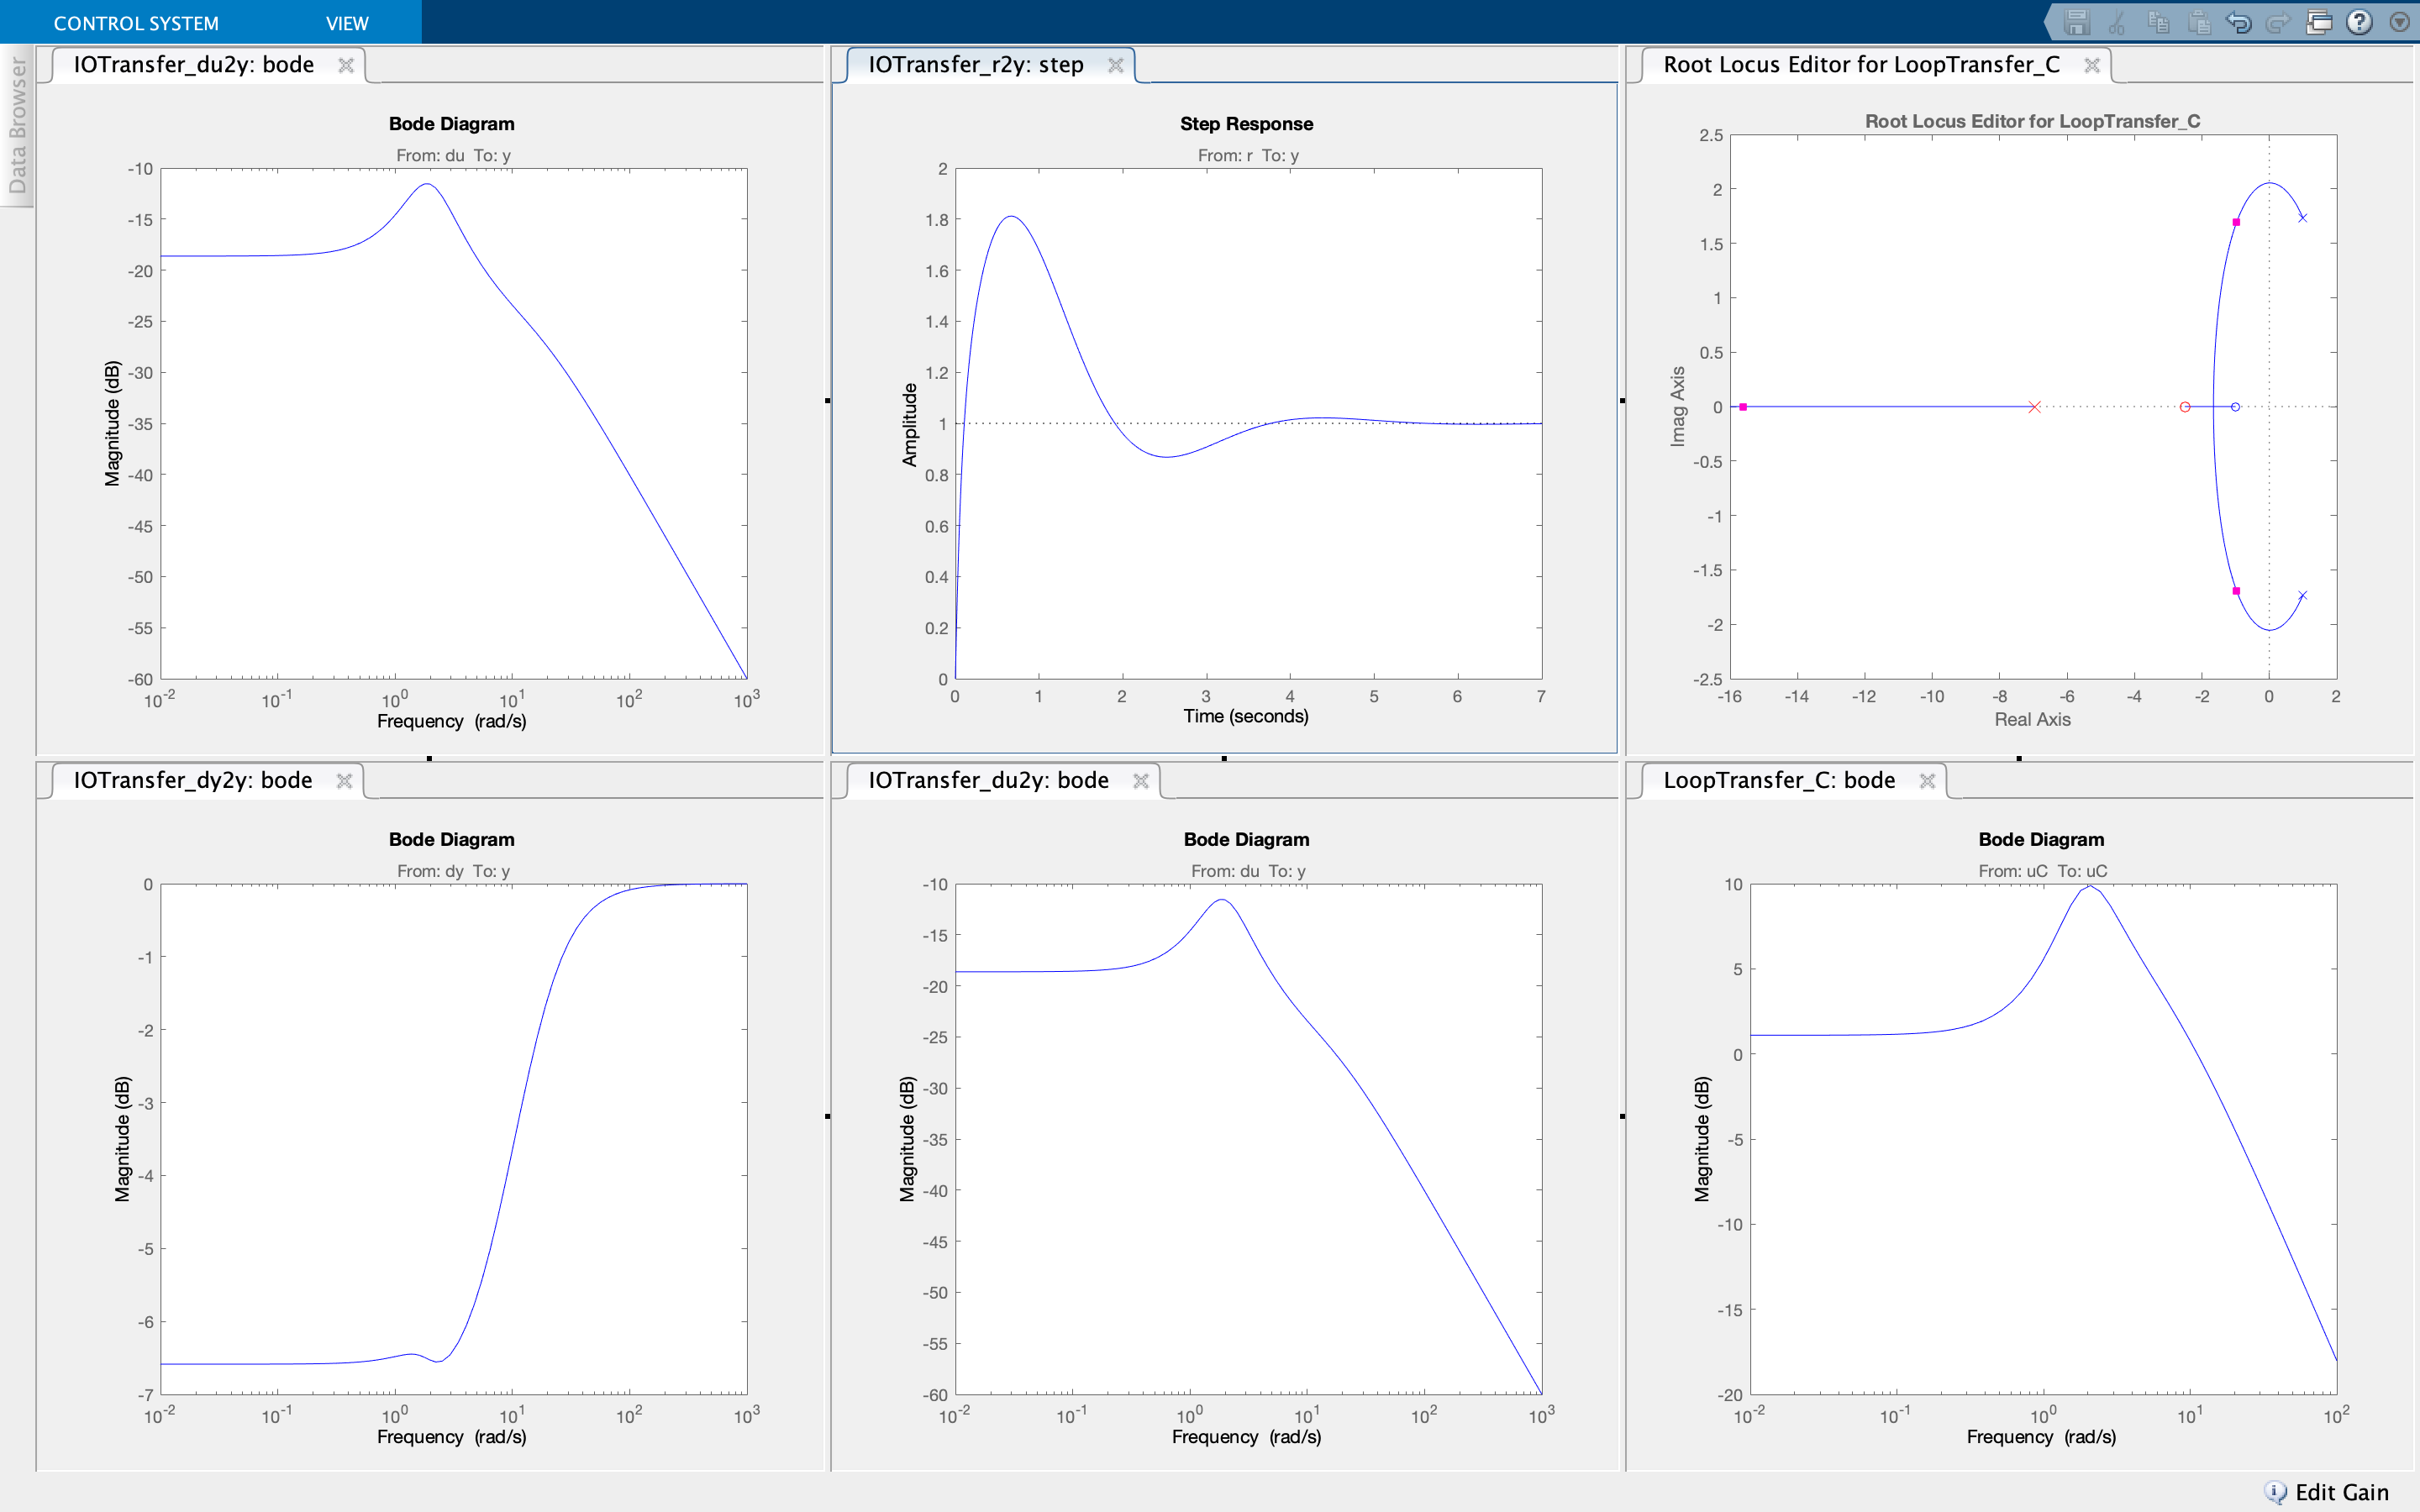
\includegraphics[width=16cm]{../Figure/Q1/Q1_c/siso_all.png}
	\end{figure}
	\newpage
	\item root locus with lead and feedforward controller
	\begin{figure}[H]
		\caption{root locus}
		\centering
		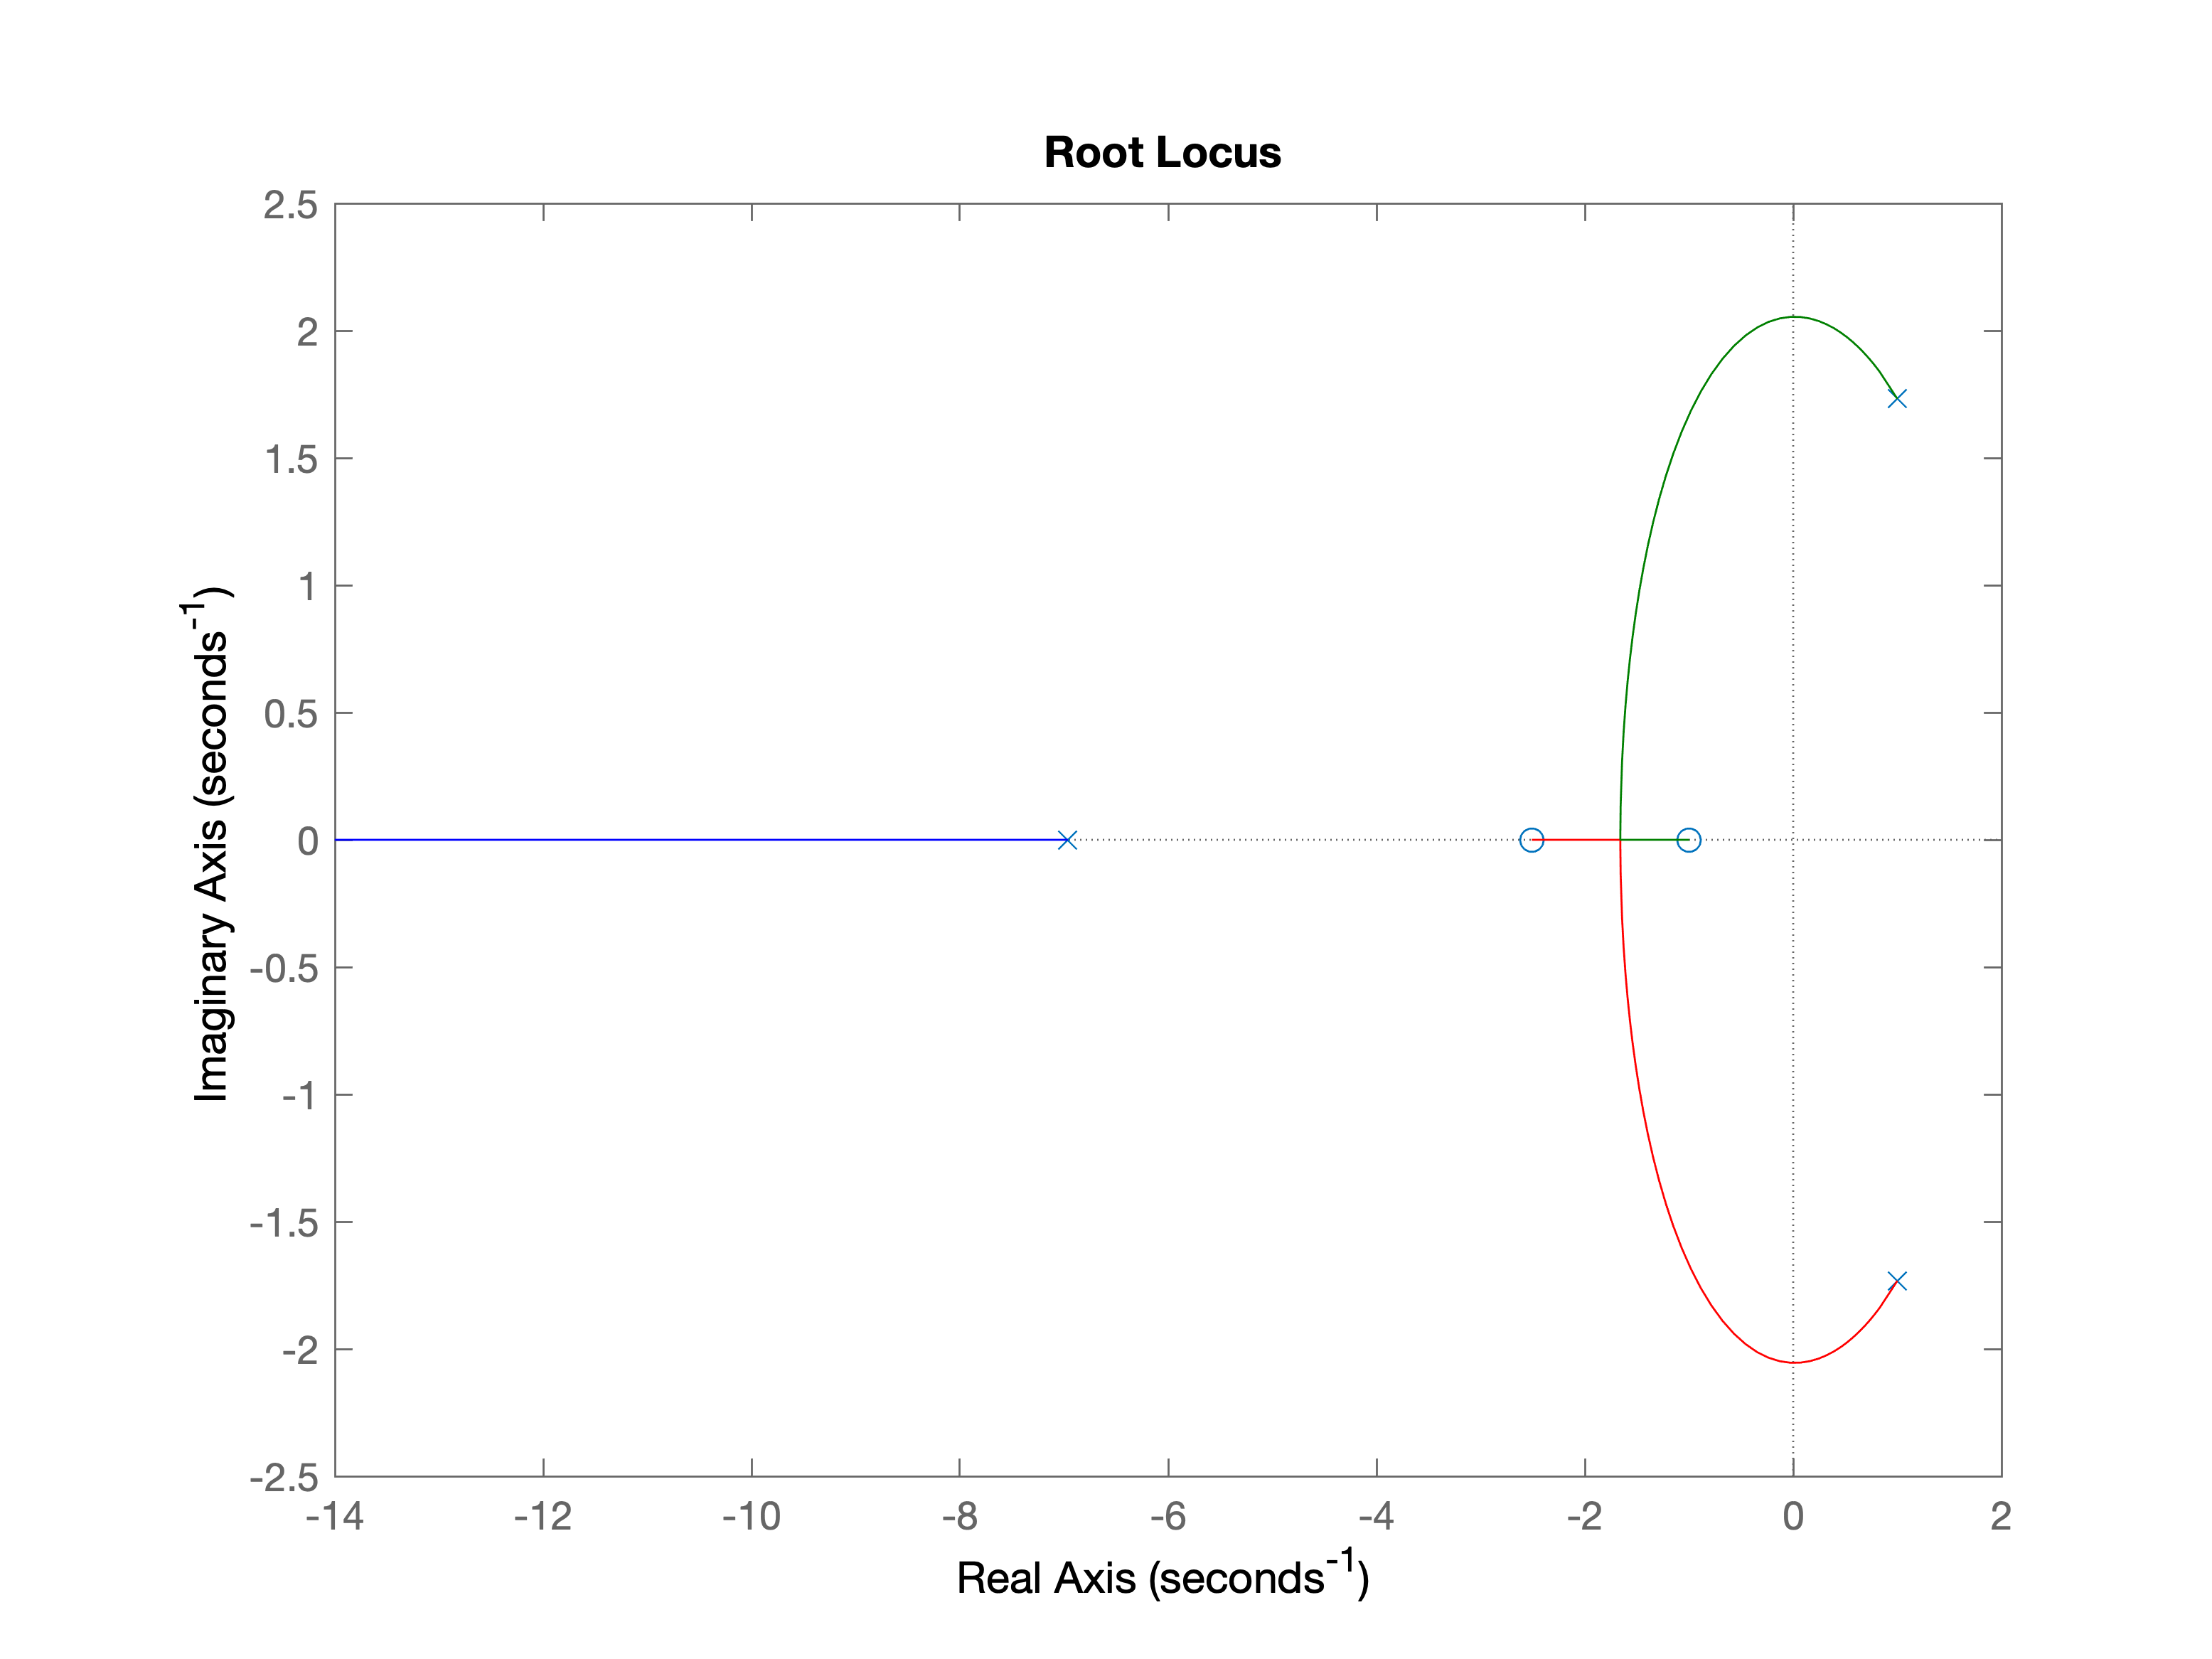
\includegraphics[width=12cm]{../Figure/Q1/Q1_c/rlocus.png}
	\end{figure}
	\item step response for closeloop system with lead and feedforward controller
	\begin{figure}[H]
		\caption{step response for closeloop system}
		\centering
		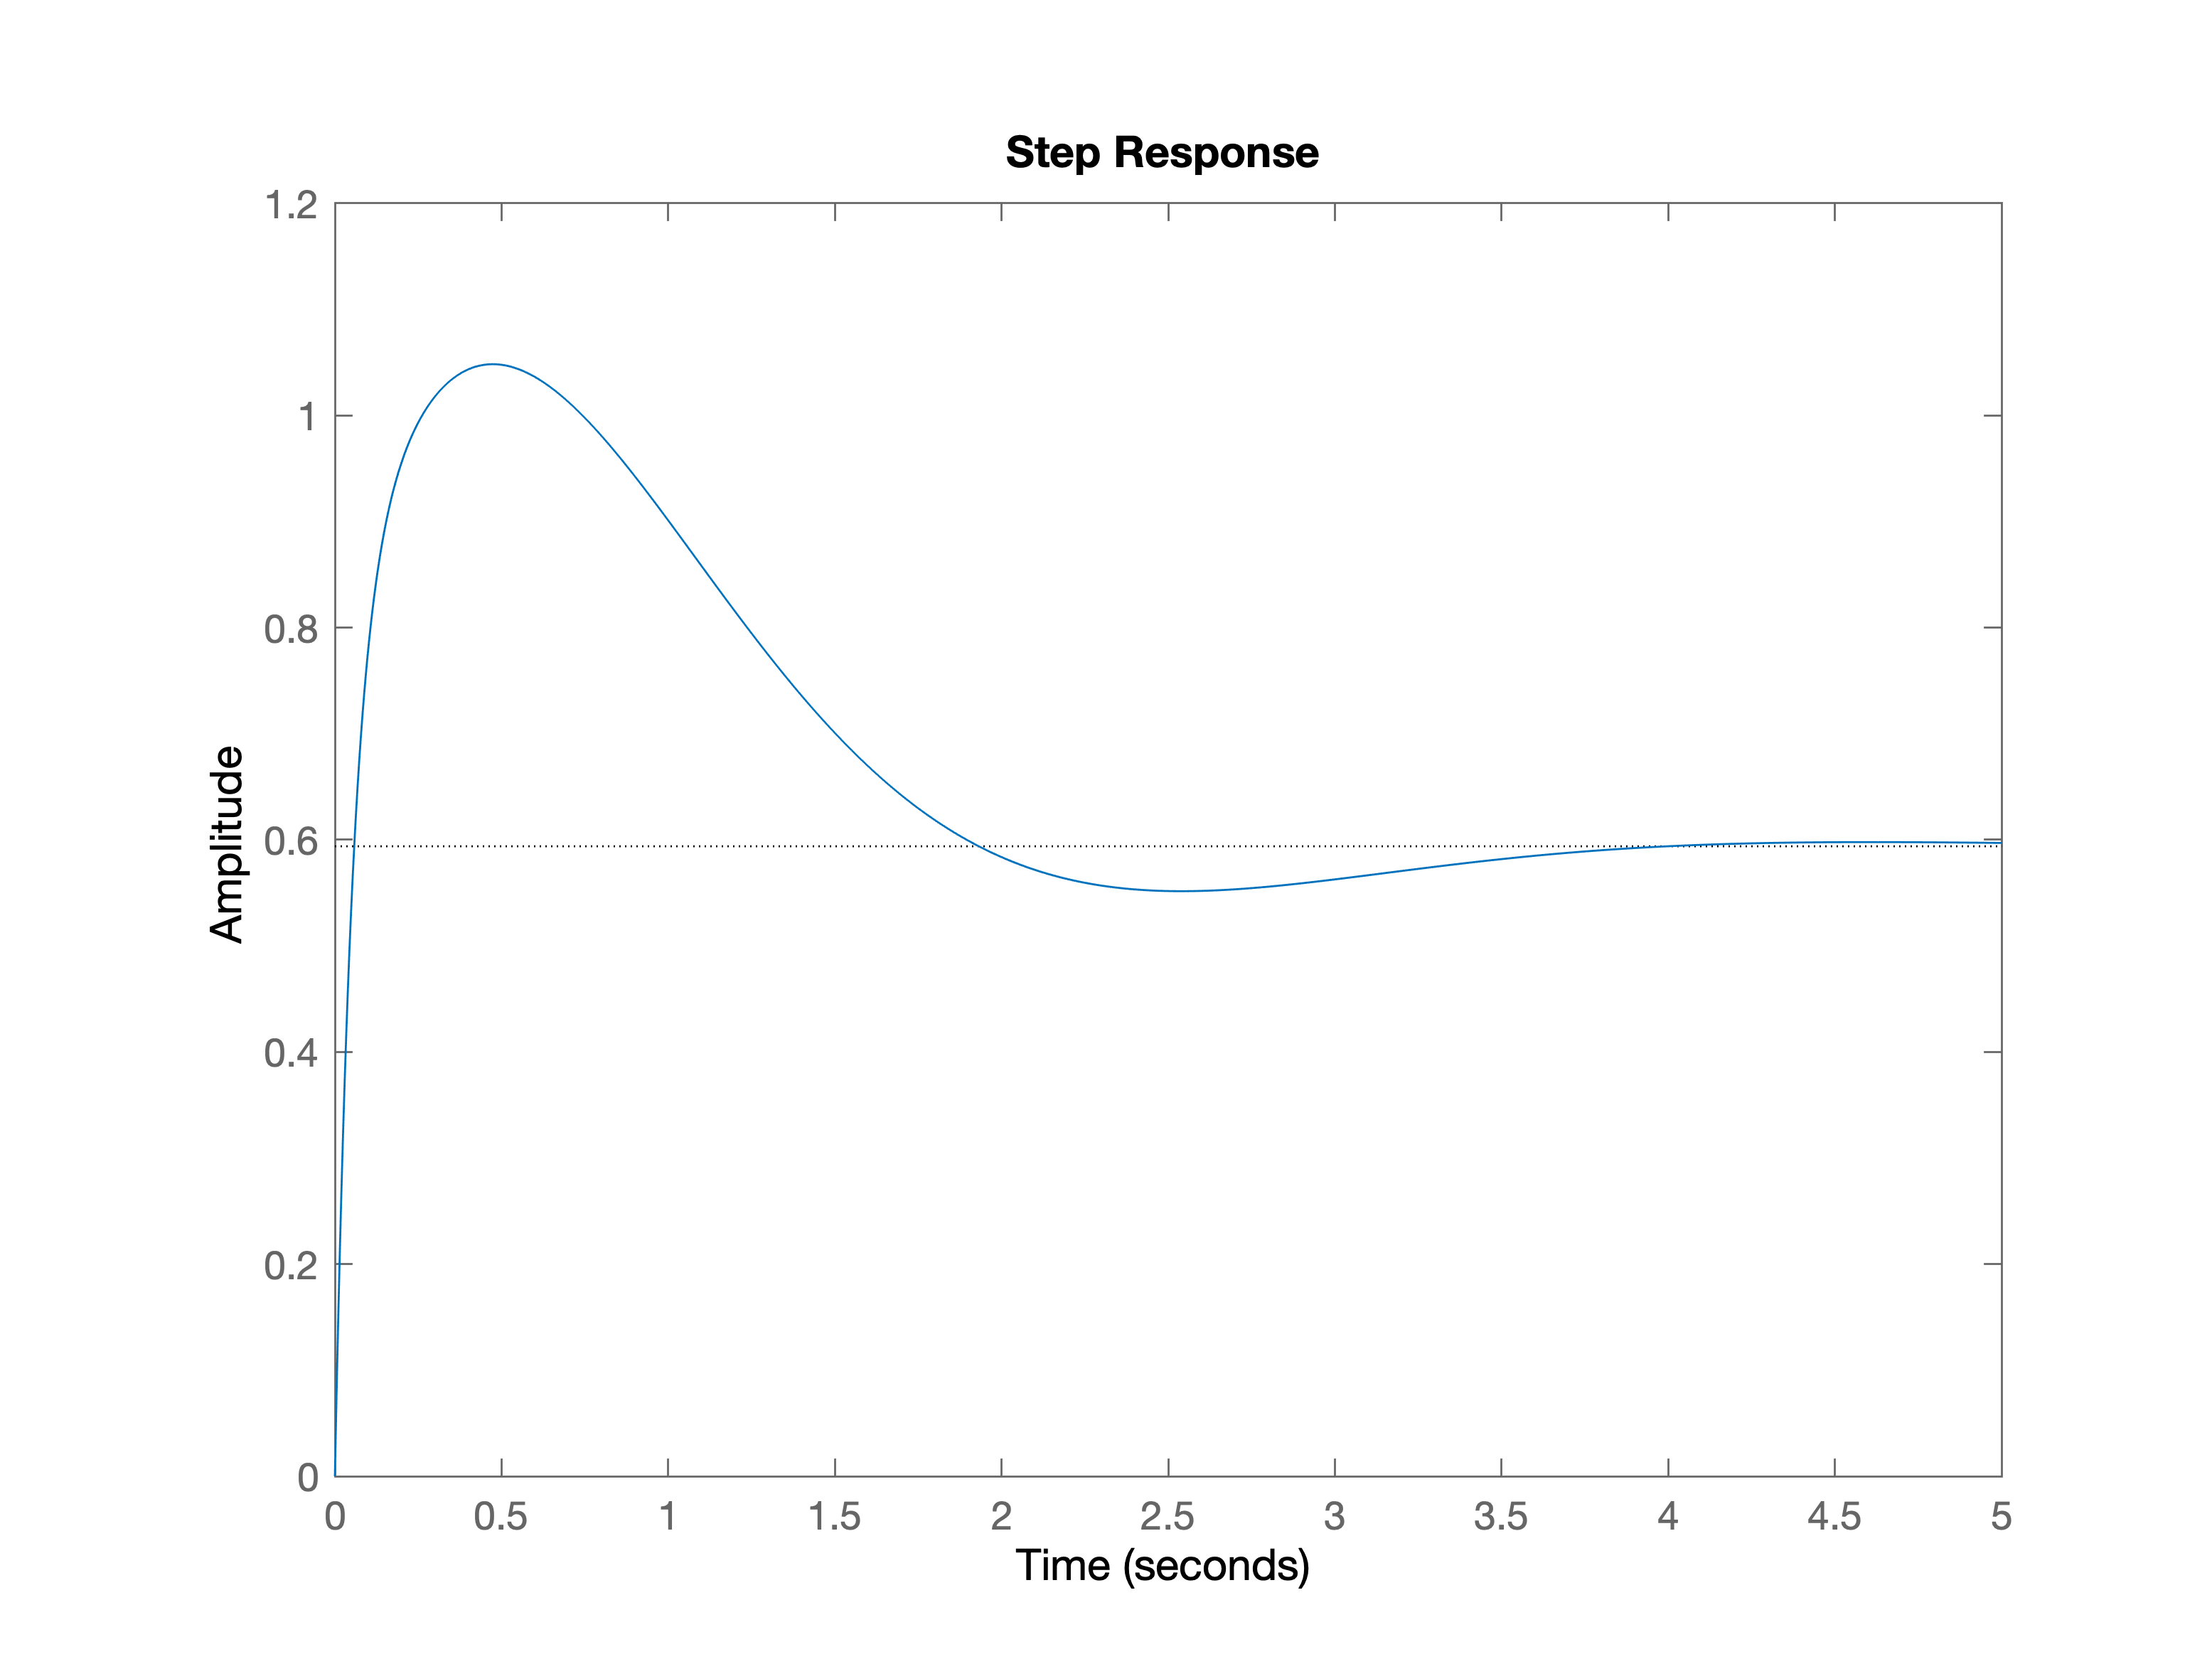
\includegraphics[width=12cm]{../Figure/Q1/Q1_c/feedback_step.png}
	\end{figure}
	\item closeloop bode (magnitude) with lead and feedforward controller
	\begin{figure}[H]
		\caption{closeloop bode (magnitude)}
		\centering
		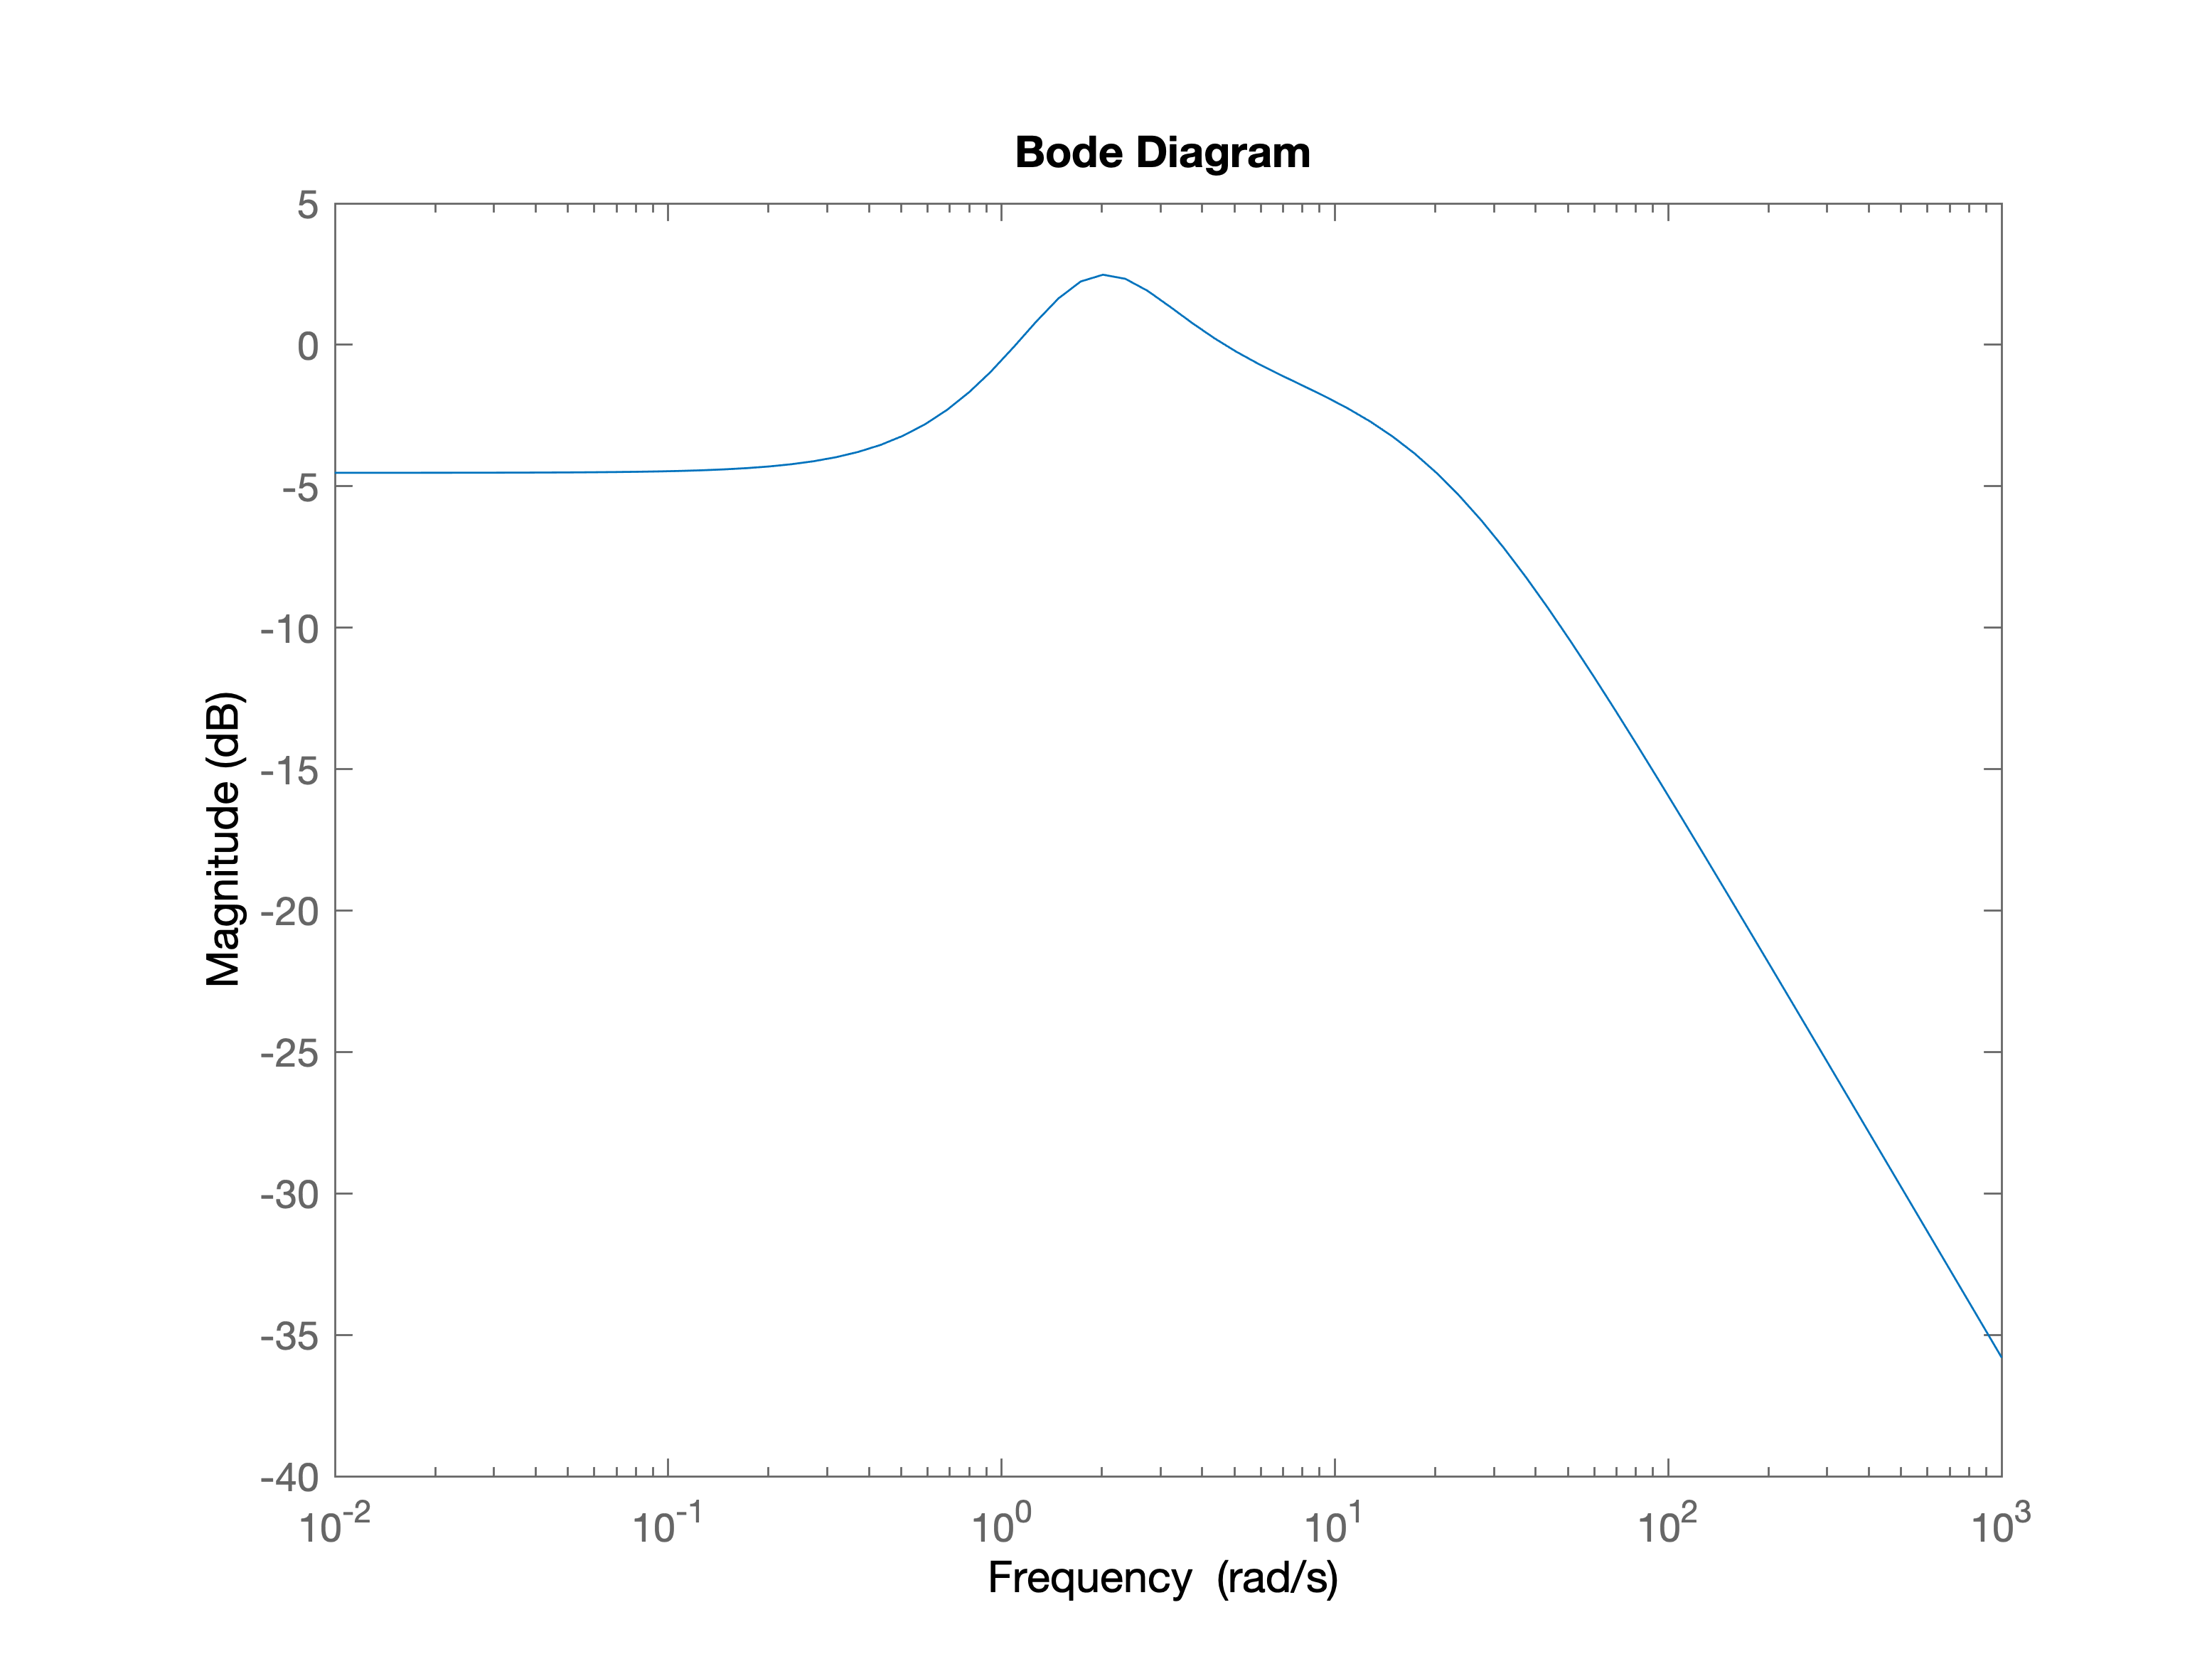
\includegraphics[width=12cm]{../Figure/Q1/Q1_c/feedback_bode.png}
	\end{figure}
	\item openloop bode (magnitude) with lead and feedforward controller
	\begin{figure}[H]
		\caption{openloop bode (magnitude)}
		\centering
		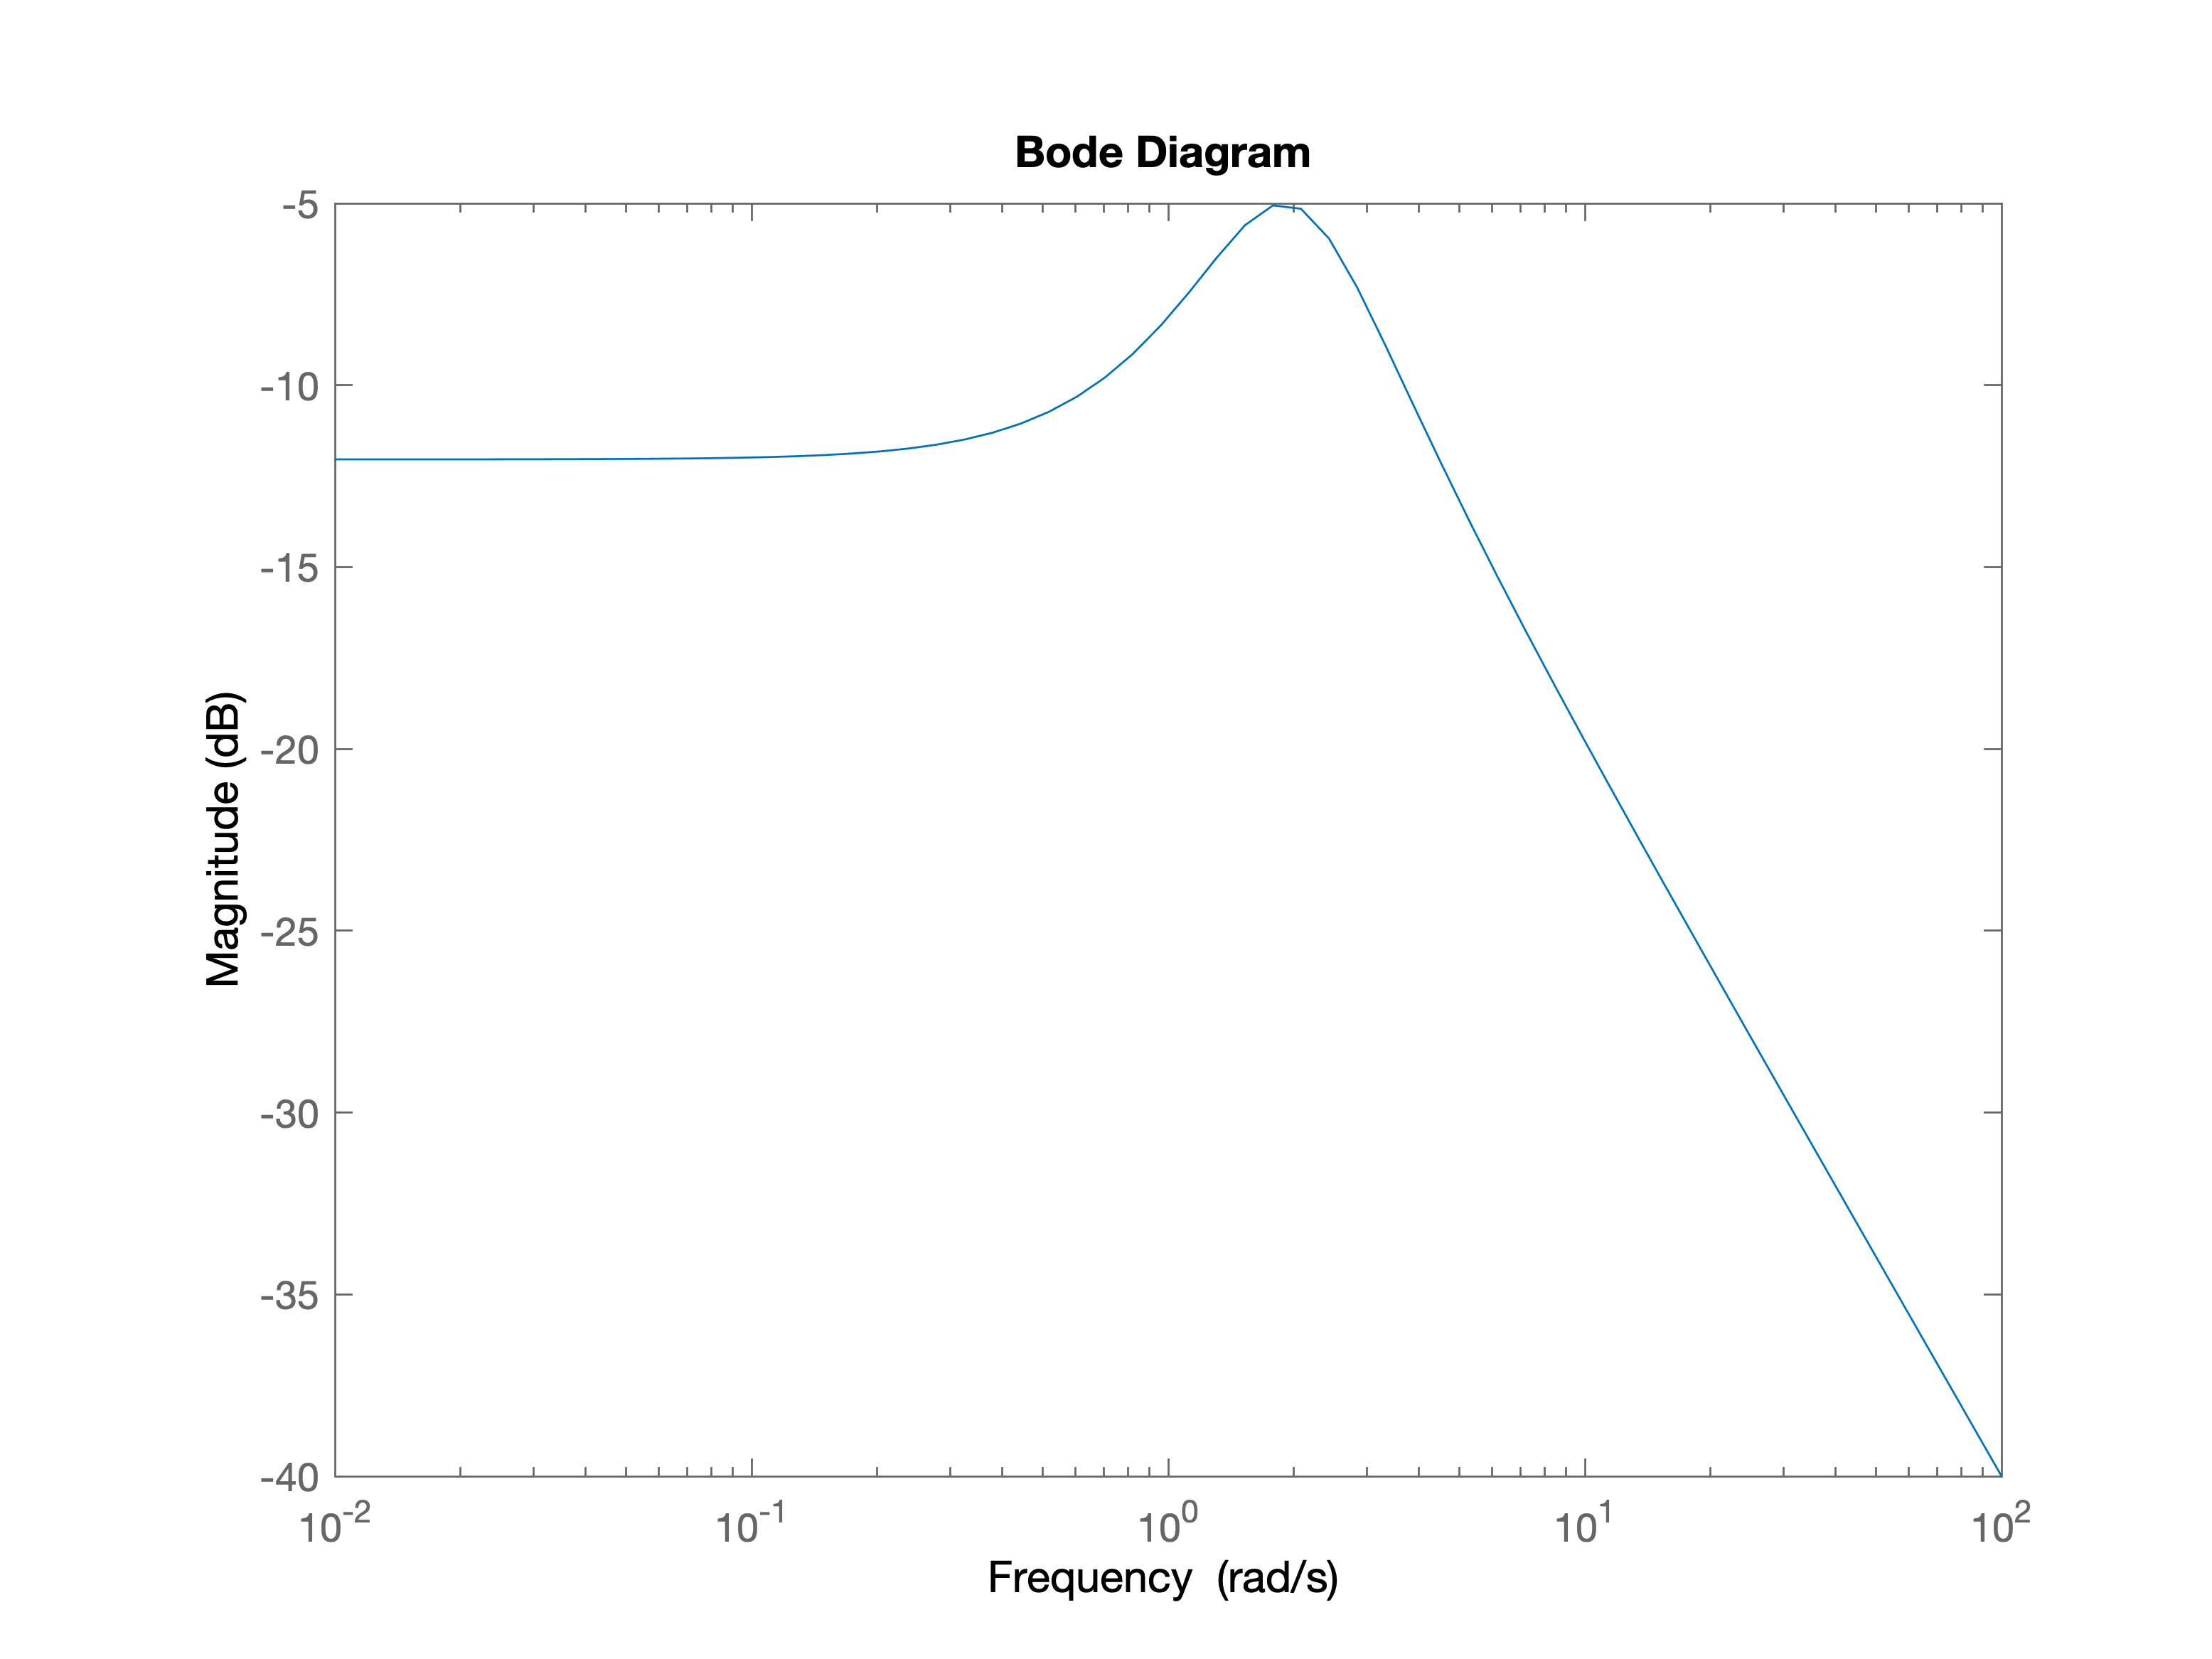
\includegraphics[width=12cm]{../Figure/Q1/Q1_c/openloop_bode.png}
	\end{figure}
	\item sensitivity function with lead and feedforward controller
	\begin{figure}[H]
		\caption{sensitivity function}
		\centering
		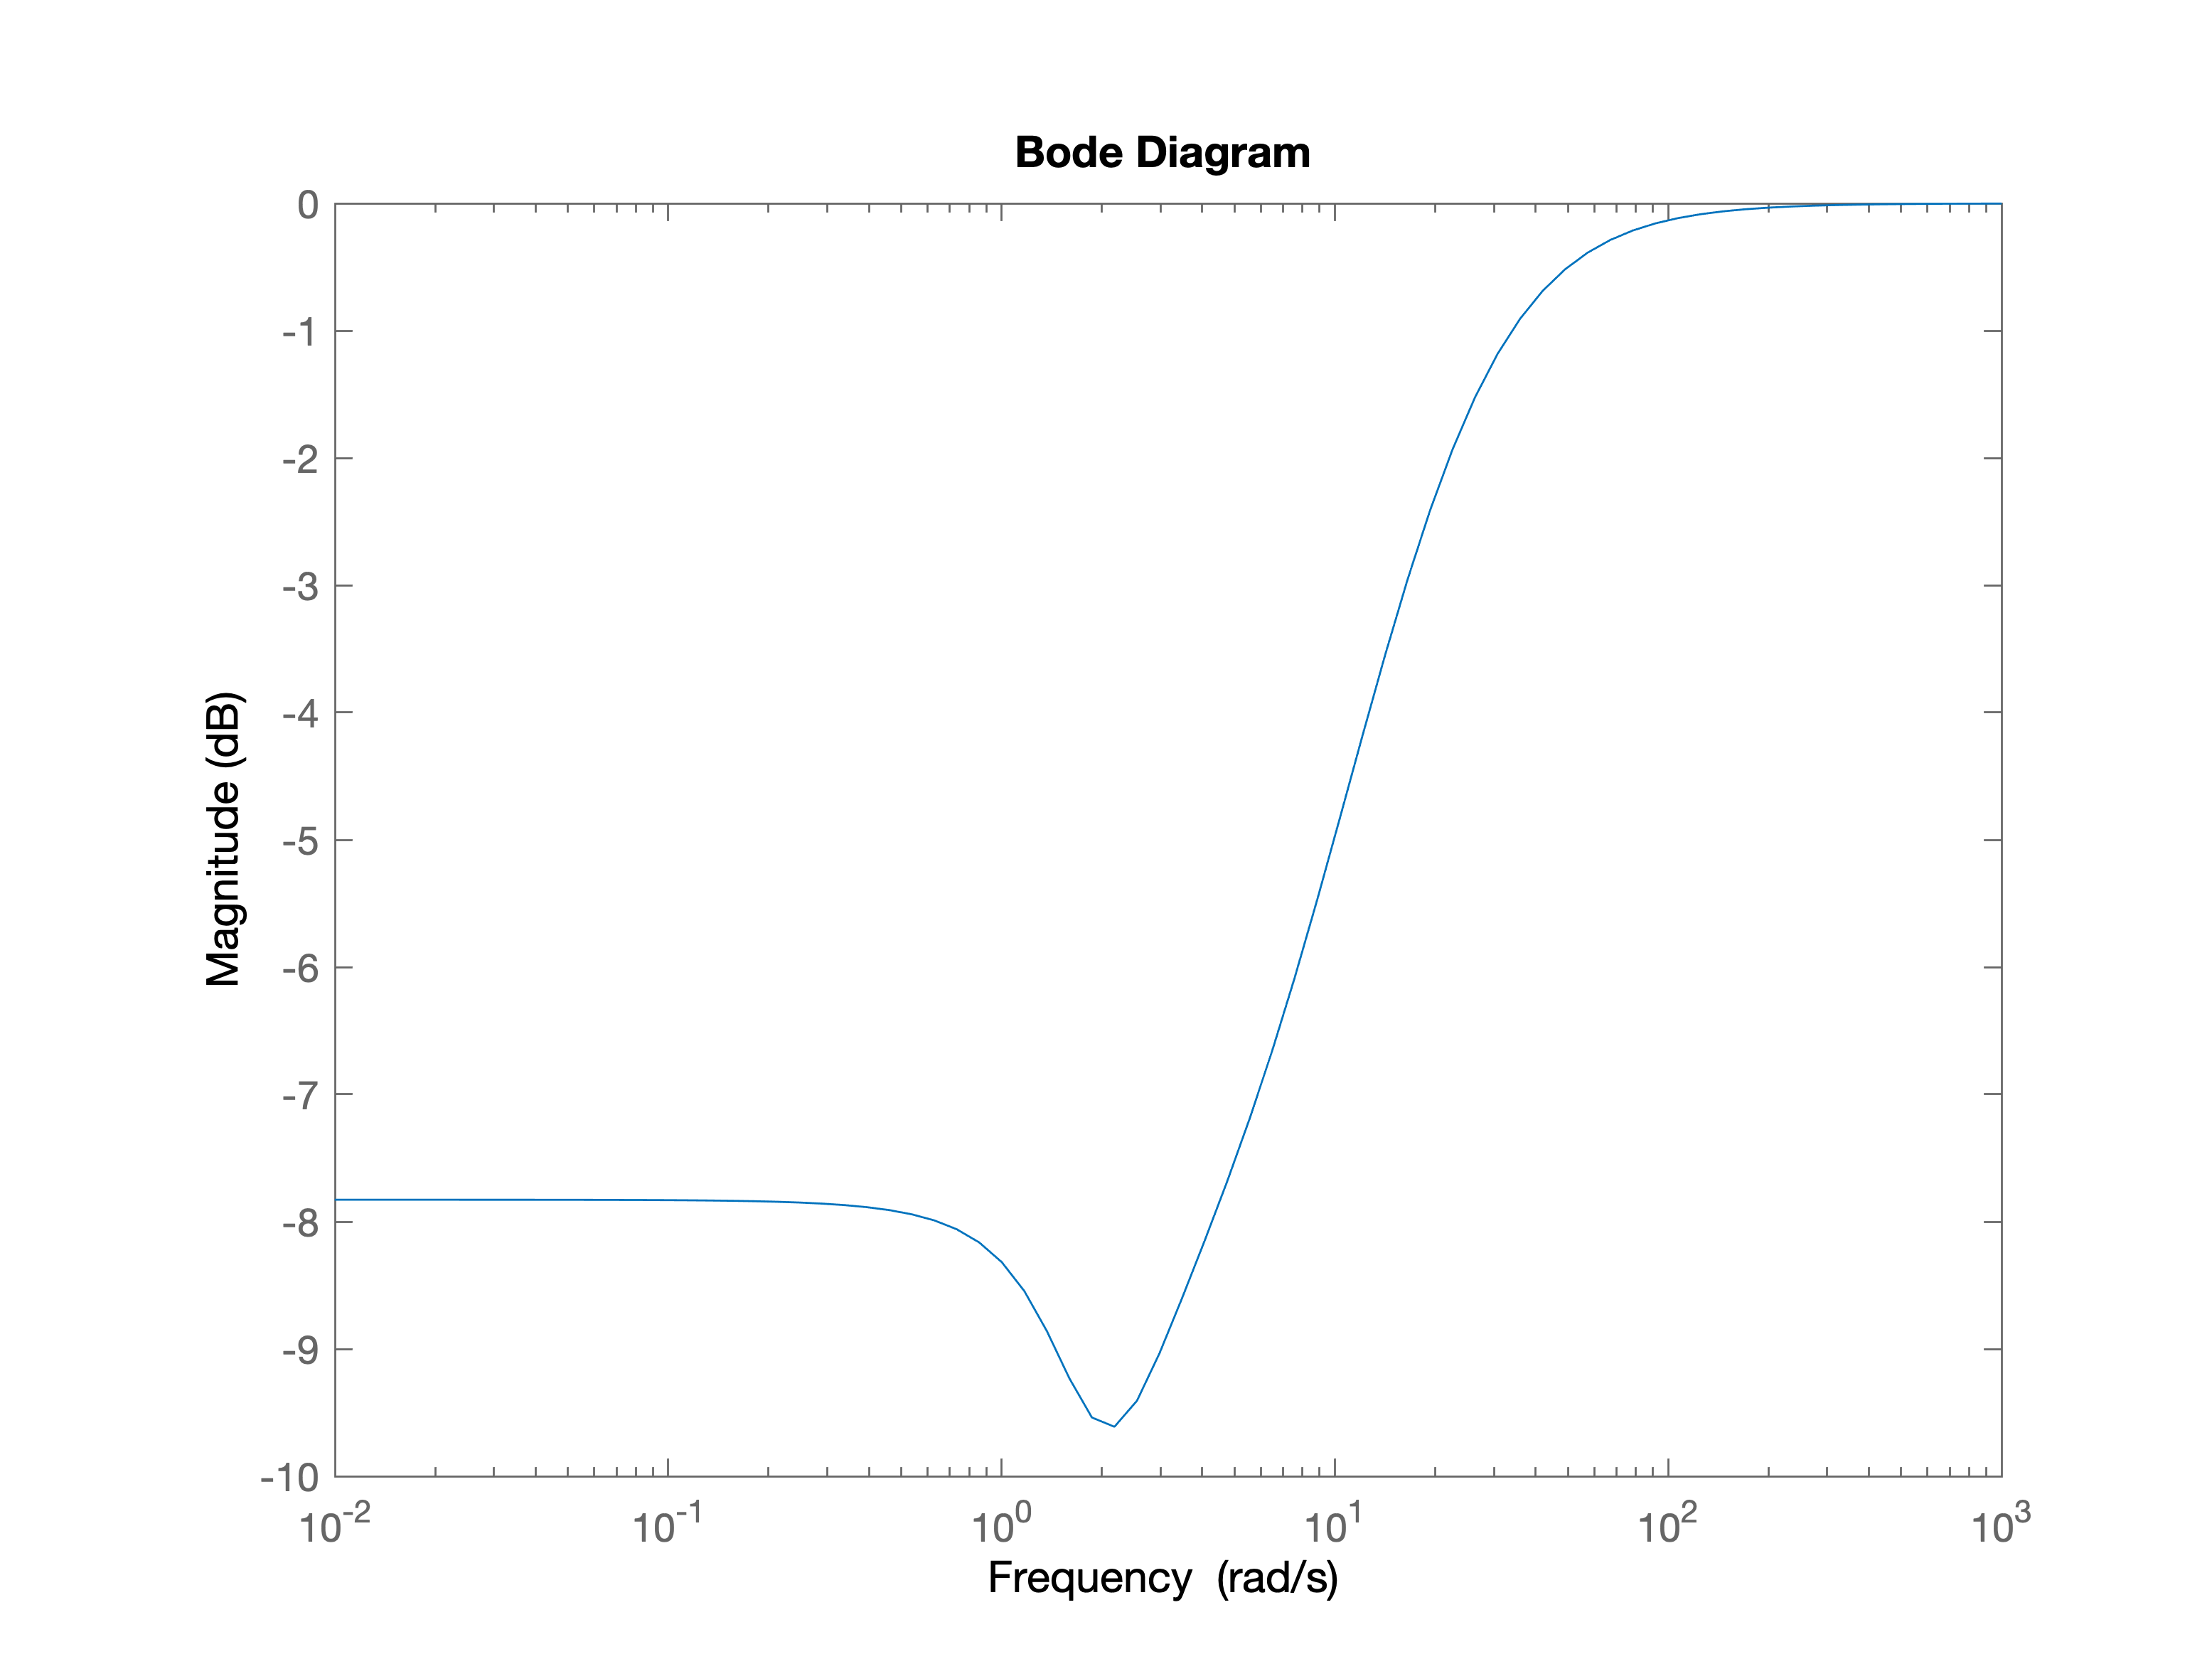
\includegraphics[width=12cm]{../Figure/Q1/Q1_c/s_bode.png}
	\end{figure}
	\item complementary sensitivity function with lead and feedforward controller
	\begin{figure}[H]
		\caption{scomplementary sensitivity function}
		\centering
		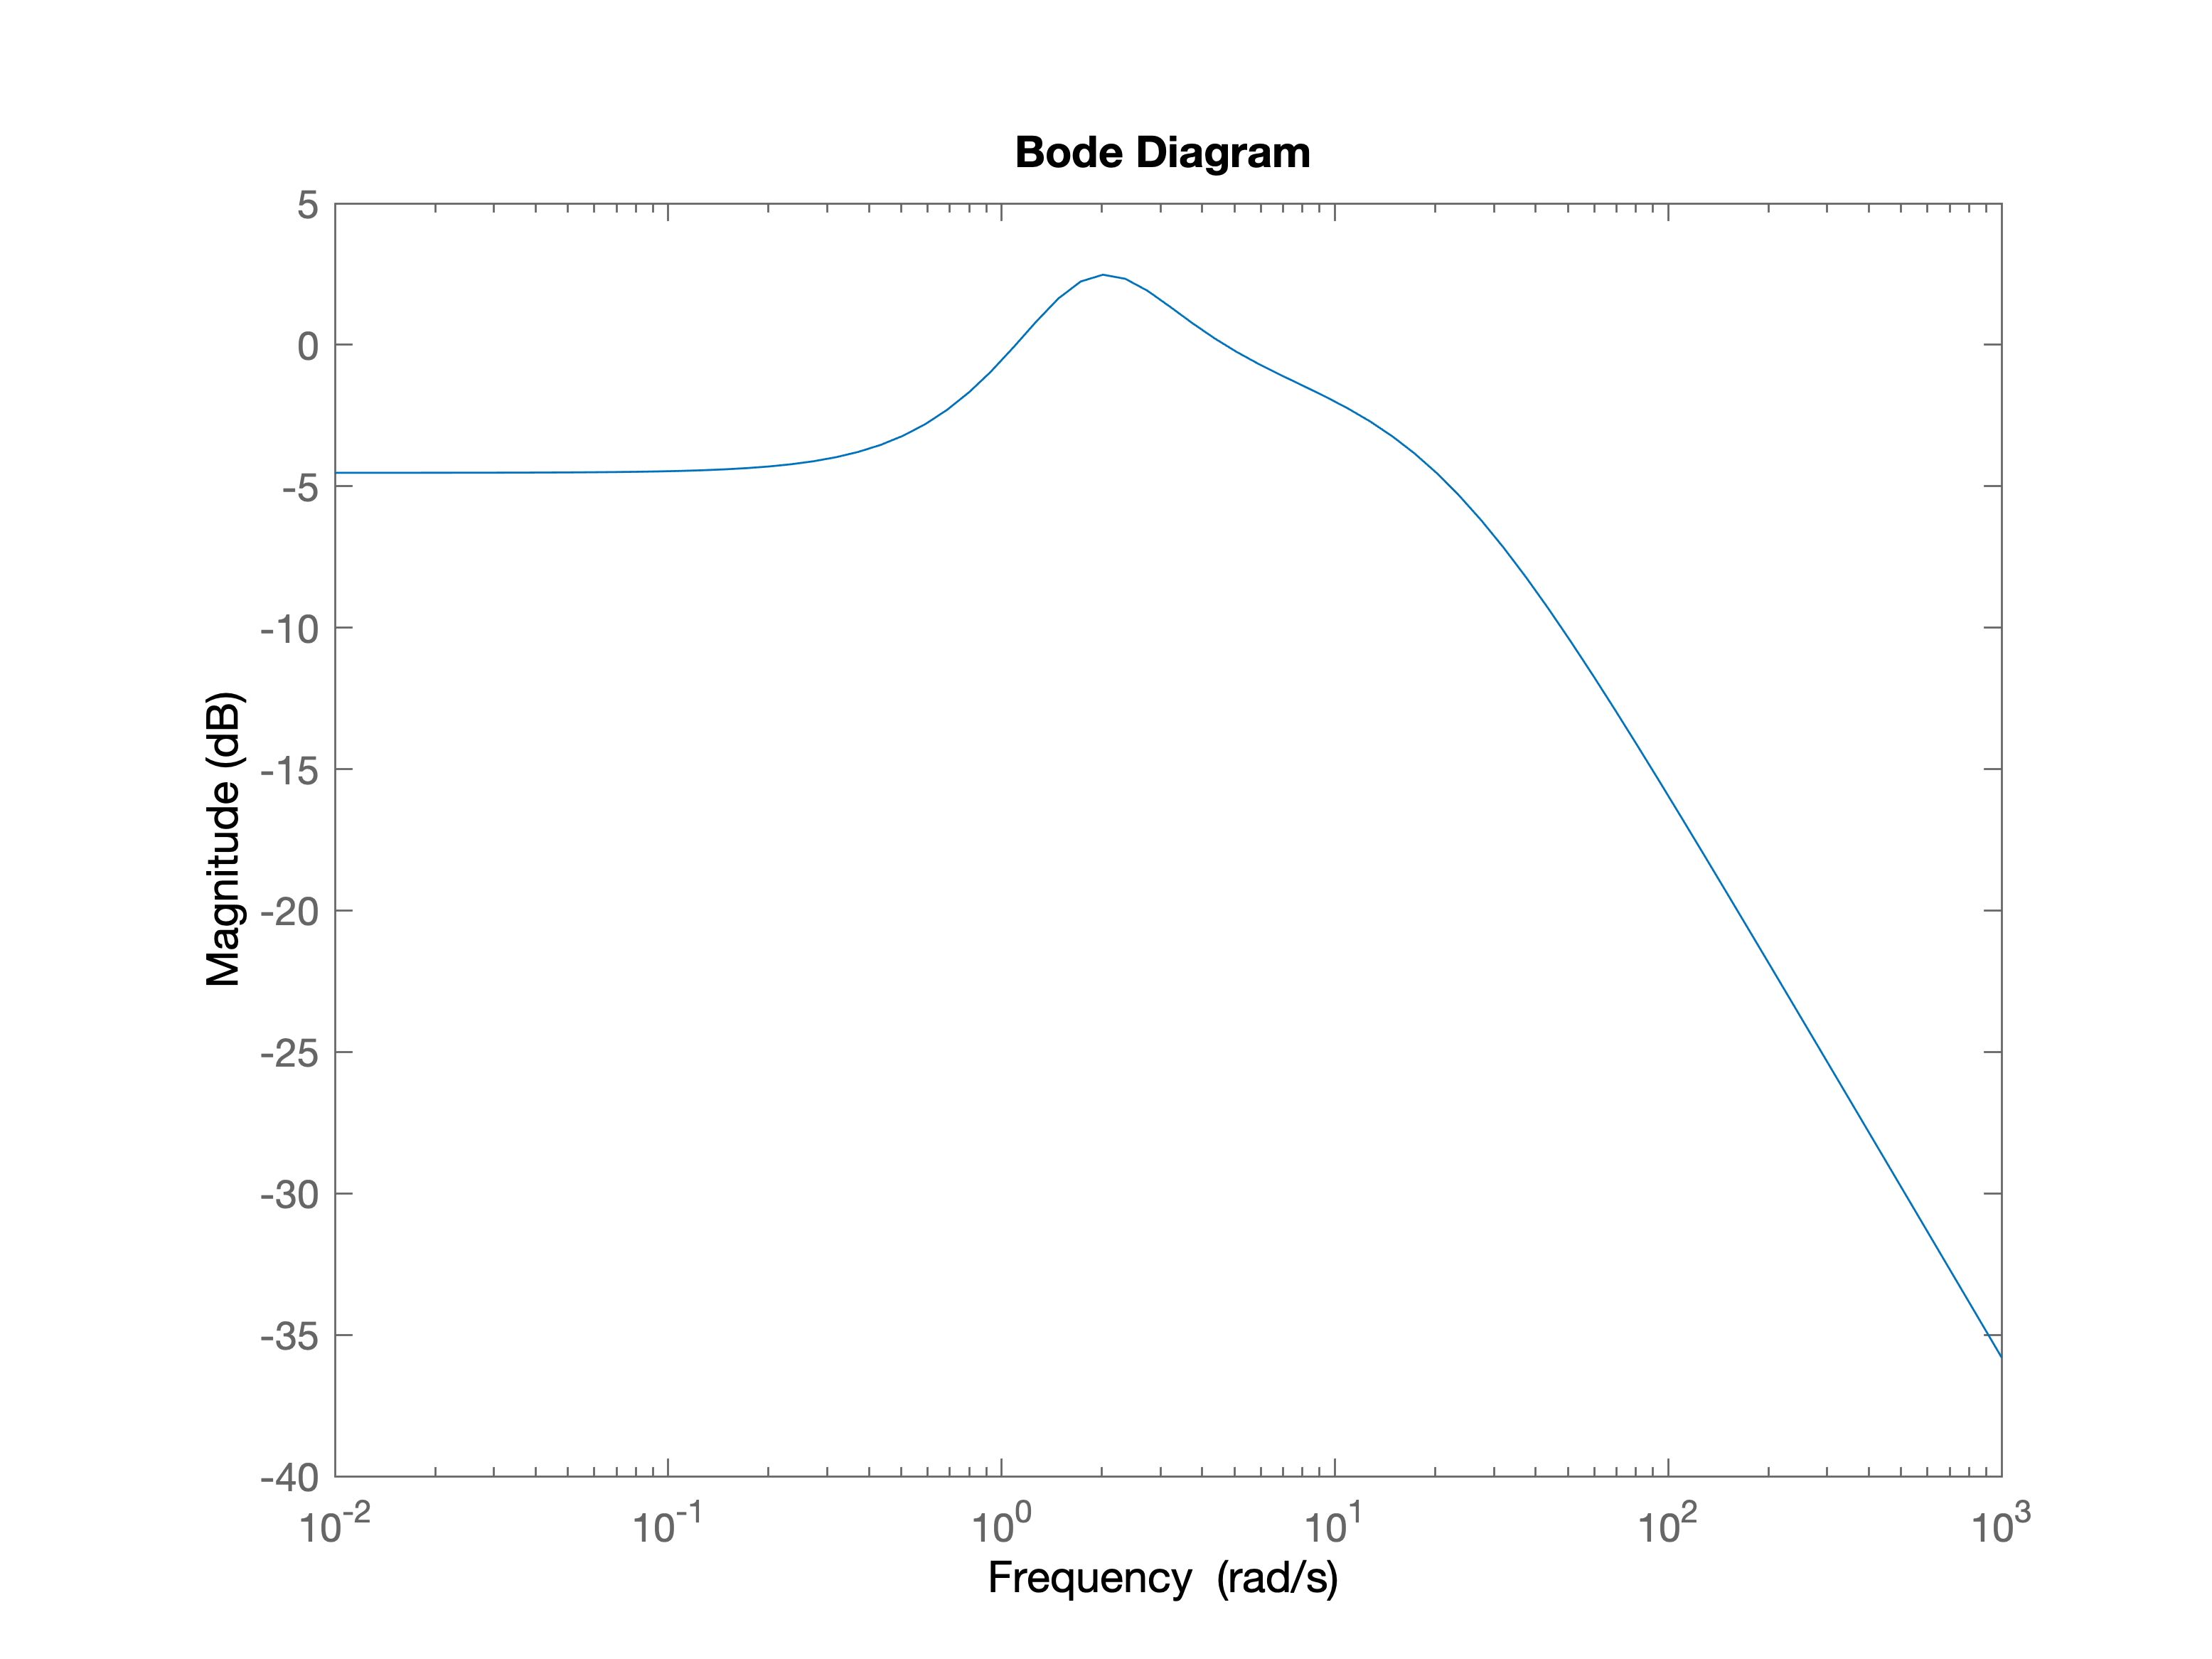
\includegraphics[width=12cm]{../Figure/Q1/Q1_c/t_bode.png}
	\end{figure}
\end{itemize}